\documentclass[a4paper,12pt,english]{article}
\usepackage[nottoc,numbib]{tocbibind}
\usepackage[utf8]{inputenc}
\usepackage[english]{babel}
\usepackage{amsmath}
\usepackage{amssymb}
\usepackage{listings}
\usepackage{hyperref}
\usepackage{booktabs}
\usepackage{graphicx}
\usepackage{makeidx}
\usepackage{titlesec}
\usepackage{fancyhdr}
\usepackage{wrapfig}
\usepackage{fancyvrb}
\usepackage{pbox}
\usepackage{hyperref}
\usepackage{mathtools}
\usepackage{amsmath}
\usepackage{multicol}
\usepackage{tocloft}%
\usepackage[refpage]{nomencl}
\usepackage{etoolbox}
\usepackage{longtable}
\apptocmd{\sloppy}{\hbadness 10000\relax}{}{}
\makenomenclature

\graphicspath{ {/} }
\pagestyle{fancy}
\setcounter{secnumdepth}{4}
\setcounter{tocdepth}{4}

%Setting link borders to none
\hypersetup{pdfborder = {0 0 0}}

\fancyhead[C]{}
\fancyhead[L]{}
\fancyhead[R]{\footnotesize{
Sebastian O. Jensen}}


\begin{document}
\pagenumbering{Alph}
\begin{titlepage}

\newcommand{\HRule}{\rule{\linewidth}{0.4mm}}
\center
\small{ \emph{Forfattere:}\\
14.06-79 Sebastian O. Jensen \textsc{GJX653}
\\
Hold 1} \\[2cm]

\textsc{\LARGE Fotonik}\\[0.5cm]
\textsc{\large DTU}\\[1.5cm]
\textsc{\huge Protocols and standards in IoT}\\
\HRule \\[0.7cm]
{\bfseries Keywords: ZigBee, Mesh networking, IEEE 802.15.4, MQTT-SN,
TI CC2530, IAR Workbench, Nodejs, MongoDB, FlipDots, Raspberry pi,
REST}\\[0.4cm]
\HRule
\\[1.5cm] \textsc{\Large \textsc{\today}}\\[0.5cm]



\end{titlepage}
\tableofcontents

\pagenumbering{arabic}
\section{Introduction}	
\subsection{Abstract}
Forecasts say that in 2020 there will be 25 Billion devices connected to the
internet. In 2014 it was estimated to be 3.7 Billion devices\cite{Gartner}.
This put a big demand on common tehnologies such as wifi, http, relational
databases, etc. This project investigate how to deal with these challenges by
building a prototype of a system that meets these challenges. The system
consist of multiple devices which connect in a local network and are made
availerble via the internet. This is a fully realistic example of how to deal
with the futura of IoT\nomenclature{IoT}{Internet of Things}. The
application consist of some battery powered devices that communicate wireless
via the ZigBee protocol, a ZigBee/internet gateway and an application server
where the backend, a database and a webportal is implemented. This report will
focus on the devices, ZigBee protocol, gateway and communication between the
gateway and application server. The report will losely touch the design of the
application server.

\subsection{Overview of this report}
In section 1.3 is the bacground for the system described. Section 2 will give a
Theoretical background on some of the technologies which will be used
to implement the system. Section 3 will give a technical description on the
implementation of the system and section 4 contains the conclution. I is
sugested to read 
\subsection{Background}
Internet of Things is the term that describes networks of physical devices that
are connected to the internet. This can be anything like sensors, whearabels,
fridges, heating systems, lightballs and what ever you else could imagine. As
mentioned there is a high growth in the number of these devices. This project
is about solving a common problem in lesure harbours. 
In leisure, harbors there are a limited number of moorings. Therefor each boat
owner has his own mooring space. At each mooring space there are a sign which
can be set to red or green. When the owner leave the harbor he should set the
sign to green indicating that the mooring is free to use for guests. If he is
away for less than a day he can set it to red indicating that the mooring is
not free to use. When the owner returns home after some days he call the harbor
master who then flip the sign to red indicating that the mooring is no longer
free. A common problem is that the boat owners often don’t set the signs to
green when they leave the harbor. The reason is it is easier to let it stay red
instead of calling the harbor master when returning home. This often result in
many unused moorings has red signs and make it difficult for guests to find
free moorings. Another problem is the time the harbor master use on flipping
the signs for people returning home to their berth.
To solve these problems a system of electronically controlled signs is
suggested. For more details about the sugested system refer to section 3.1




\clearpage
\subsection{Abbreviations}


\renewcommand{\nomname}{}
\renewcommand{\pagedeclaration}[1]{}
\pagestyle{empty}
\printnomenclature[3cm]
\clearpage



\section{Theroretical background}
\subsection{Wireless networks}
Their exist many different wireless communication standards today all serving
different purpose. There is the IEEE 802.11 specifications which define
different protocols used for implementing WLAN which we mostly use for
connecting our computers and smartphone to the internet. Then there are the
mobile networks such as GSM, EDGE, UMTS, HSPA, etc. Which are used by phones to
send voice or internet data. Some less know technollogies include AIS
\nomenclature{AIS}{Automatic Identification System} which is used to transfer
data between commercial ships over VHF and satelite. They all have different
purpose and theirfore also different demands. Eg. When handling voice calls
over the mobile network the latency should not be to high and the protocol
should suport the devices in using as litle power as posible. Here follow a list
of important factors to consider when choosing a wireless tecnology.
\begin{itemize}
  \item Bandwide
  \item Latency
  \item Power consumtion
  \item Maximum number of nodes in the network
  \item Range
  \item Reliability
  \item Cost
  \item interoparebility 
\end{itemize}

For the purpose of this project we will later see that the
ZigBee Standard is a good solution for communicating with the signs in the
harbour.

\subsection{ZigBee}
\subsubsection{Overview}
ZigBee is a standard used to connect devices. It is managed by the ZigBee
allianze which count mebers such as Texas Instruments, Philips, Silicon
Labs, NXP, Samsung and many more. ZigBee aims at being relierble, secure,
lowpower and easy for the consumer to use. ZigBee specify all the layers
in the OSI-model\nomenclature{OSI-model}{Open System Interconnection Reference
Model}. There exist different version of the ZigBee protocol. But this project
is bassed on the ZigBee Pro standard. In the rest of the report refering to the
ZigBee standard it should be asumed it is the Pro version.

\subsubsection{Layers}
\paragraph{ZigBee layers}
ZigBee is build on top of the 802.15.4 standard which define the PHY and MAC
layer. Therefore these layers are not defined by but implemented by
ZigBee.
On top of 802.15.4 ZigBee define the layers all the way up to and including
the APL. The layers communicate via Service Access Points
(SAP)\nomenclature{SAP}{Service Access Point}. An overview of the ZigBee
model and the SAP that makes the services availerble between
them are shown in figure from the ZigBee Alliance in fig. 1. below.
\begin{figure}[h]
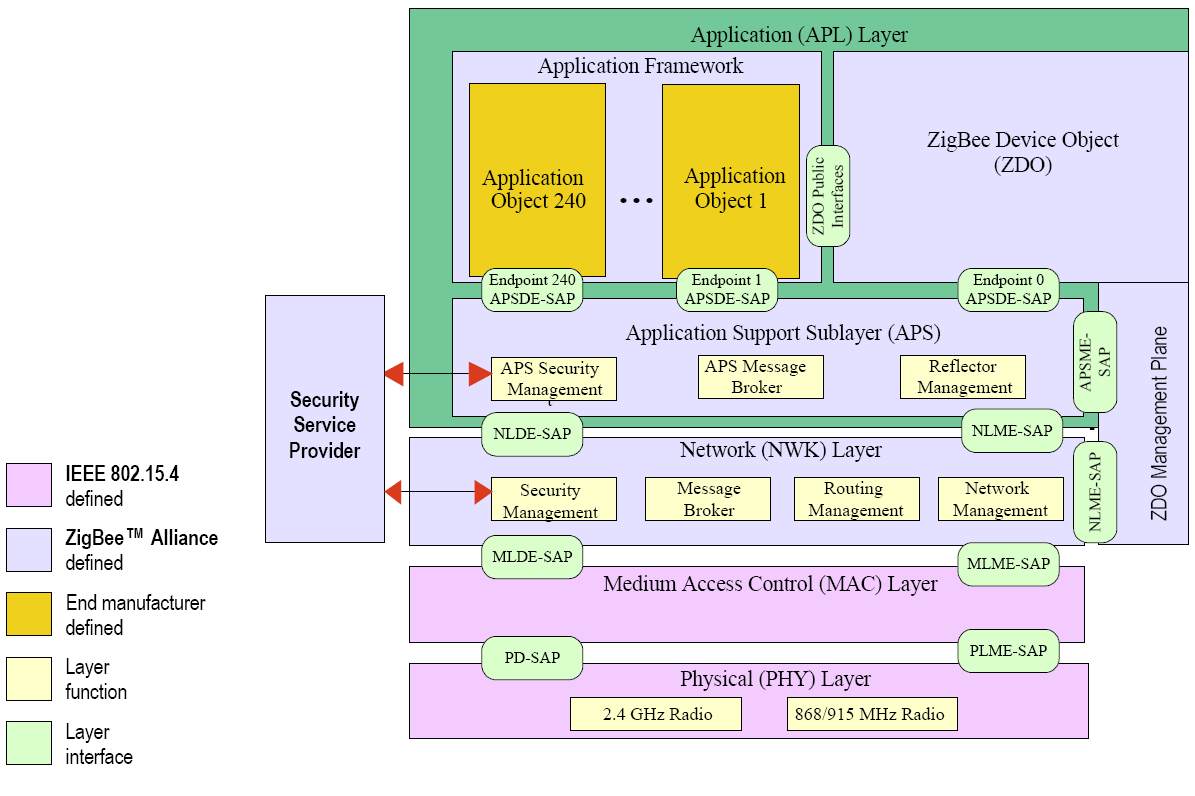
\includegraphics[width=\textwidth]{zigbeeLayers.png}
\caption{ZigBee Model\cite{zigbeeModel}}
\end{figure}

\paragraph{802.15.4}
The 802.15.4 standard specify the 2 lowest layers PHY and MAC. 802.15.4 specify
three types of roles. These roles are named a litle different in ZigBee. See fig
2 for a list of the roles in 802.15.4 and their corsponding ZigBee names. In this section (2.2.2.2) we will use the 802.15.4 names 

\begin{figure}[h]
\begin{center}
\begin{tabular}{| l | c |}
  \hline
  802.15.4 role & ZigBee role\\
  \hline
  PAN coordinator & Coordinator\\
  \hline
  Coordinator & Router\\
  \hline
  Device & End Device\\
  \hline
\end{tabular}
\end{center}
\caption{802.15.4 and ZigBee device roles}
\end{figure}

There can only be one PAN coordinator \nomenclature{PAN}{Personal Area Network}
in a network. The 802.15.4 Implement star networking where the Devices can
be connected to exactly one coordinator and the coordinators can be connected to
other coordinators and multiple devices. see fig 3
-------------------------------------------------- 
\subparagraph{Physical (PHY)\nomenclature{PHY}{Physical Layer}}
The PHY is responsible for the physical part of the network. This is
harware specific things like frequency, modulation, how to avoid coalition
with other devices, receiver sensitivity, output power and other hardware
specific parametters. The PHY provide service to the MAC layer via the
PLME-SAP \nomenclature{PLME-SAP}{Physical Layer Management Entity Service Access
Point}.The PHY is also responsible for the
following tasks
\begin{itemize}
  \item Selecting the frequncy
  \item Turning on or off the transiver
  \item Perform Energy Detection. This can be used by the coordinator to find
  the channel with is least bussy to use for the network.
  \item Generate Link Quality Indication (LQI) \nomenclature{LQI}{Link Quality
  Indicator}
  \item Performing clear channel assesment (CCA)\nomenclature{CCA}{Clear Channel
  Assement} which is used to detect if there is other transmision happening.
  \end{itemize}
  
\subparagraph{Medium Access Layer (MAC)\nomenclature{MAC}{Medium Access Layer}}
The mac layer provide service to the NWK layer via the MLME-SAP
\nomenclature{NLME-SAP}{Network Layer Management Entety Service Access Point}.
The MAC layer has the following responsibilities:

\begin{itemize}
  \item Generate the becons if the network is becon enabeled.
  \item Syncronisation of the devises with the becon messages
  \item Implement CSMA-CA
  \item Keep control of when the device has its GTS
  \item Perform relierble transfers between to notes
  \item Support security if enabeled 
\end{itemize}
To avoid coaltion with other devises ZigBee can use two different mekanismes.
The first methode completly relly on a tecnics called CArrier Sense Multiple
Access with Collition Avoidance (CSMA-CA)
\nomenclature{CSMA-CA}{Carrier Sense Multiple Access with Collition Avoidance}
which basicaly means that the device listen for a carrier before transmiting. If
a carrier is sensed the device back of for a set time and then try again. In the
other method the coordinator assigns a garantied time slot
(GTS)\nomenclature{GTS}{Garantied Time Slot}to a device.
If the device has been assigned a GTS it will transmite doing that time slot.
All the time slots that are being assigned are happening doing the Supper
Frame. The supper frame is simply a time period where the time slots are
assigned. Before/after the supper fram the devices that has not been assigned a
GTS can transmit using the CSMA-CA. For this method to work all the devices
requires to have the clock syncronised. Therefore this method require that the
devices wake up oftent to syncronise the clocks by listening to becons send from
the coordinator. This methode is therefore not used so often when there is a
high demand for low power consumtion.

Transfers from a device to a coordinator is simple. The device simply sent the
data either doing its garantied GTS or with CSMA-CA. The device can specify
if it want an Acknowledgement (ACK) from the
coordinator \nomenclature{ACK}{Acknowledgement} but that is optional.

When a coordinator has data for a device it can not just send it
imidiatly as the device might be a sleep. So the coordinator keeps the data
until the device ask for it. What happens is the following.
\begin{itemize}
  \item The device Periodicaly or every time it wakes up sends a data request to
  the coordinator.
  \item When the coordinator recives the data request it sends an ACK with
  indication that there is pending data.
  \item Right after the ACK has been send the coordinator start sending the
  data.
  \item The device first receives an ACK with data indication and then know it
  should expect incomming data. So it waits for the data and if indicated by the
  coordinator the device sends an ACK.
\end{itemize} First the device

If the device sends a data request and there is no pending data the coordinator
will send back an ACK with a no data indication and the device can then go back
to sleep.

\paragraph{Network Layer (NWK)\nomenclature{NWK}{Network Layer}}
The NVK is specified by ZigBee and therefore the ZigBee names will be used
to specify the dive roles. refer to fig. 2. The NVK layer is the heart of the of
the ZigBee protocol. It is in this layer the core features which makes ZigBee
speciel is implemented. The NWK layer are responsible for the following

\begin{itemize}
  \item Seting up a device as Coordinator, Router, or End device
  \item Forming the network and implement tree or mesh topology
  \item Association and assigning adresses
  \item Route discovery and maintanense
  \item Routing messages
 \end{itemize}

\subparagraph{Network topology}  
The topology of a ZigBee network can be either tree or mesh. In tree topology
there is a hierarchi between the devices. A device can only communicate with its
parrents and childs. In contrast to the tree topology is the mesh topology. In a
mesh topology any device can contact other devices. eg. if the responsible
router of and End device breaks down the device will then try to connect to
another router if there is any within its range. Also if a route is broken the
devices can then fix the route by goin other ways. This is what makes the ZigBee
network self healling. There is some few different ways the ZigBee network
can be set up which affect how routing is performed. It will be out of the
scope of this report to go true all details. Here gives an overview of how it
works using one of common settings.

\subparagraph{Routing}
Coordinator and routers create and maintain routing tables. A routing
table does not contain all information about a route, but only which
direction (to which device) a router or coordinator should send the package. The
endevice does not store any routing table. When an end device
wants to send a message it sends it to the router it is connected.
Lets asume that routes has been discovered and their by also the routing tables
has been populated with the data. Then when a router or coordinator along a
route receives a package. It look up the naighbor device to which it should send
the package in its routing table. It then forward the package to that device.
this happens until the device reach its destination. But before the this can
happen the route discovery ofcourse need to take place.

\subparagraph{Route discovery}
Only the coordinator and routers can perform route discovery. When discovering
routes the cost of the path are calculated. The route whith has the lowest cost
is choosen. When calculating the cost of a path the LQI number and number of
hops is used. There are 3 types of route discovery.

\begin{itemize}
  \item Unicast route discovery
  \item Multicast route discovery
  \item Many to one route discovery
\end{itemize}

Unicast route discovery is initiaded from the source device which sends
a broadcast route discovery to the devices in range. When the request is
received by a neighbor then this neighbor look in its routing table if it has
the route for that device. If not it sends a new route discovery brodcast
message. But before the packet is send a routing discovery table is populated
with the path cost. In this way a route discovery message can travel true the
network until it reach the destination. At the destination the cost of the route
can be obtained from the route discovery table whis whas populated when the
packet traveled along the route. The destination device will often receive more
route discovery packages with different route discoveryu tables. The destination
will then choose the route with the lowest cost and send a responce back to the
source devices and the routing tables along the way will then be updated.

Multicast route discovery is in many ways similar but instead of the destination
is one device it can be a group of devices. 

The many to one route discovery also works in similar ways as the unicast route
discovery but here the route discovery will discover routes to all devices in
the network. This is usefull when there is a central point that need to
receive messages from all the other devices.

It is posible for a device to specify the exact route when sending a
message. In this way the routing tables in the are not used. But this is not
being used in this projekt.

\subparagraph{Route maintenence}
ZigBee is self healing. This means that if a route gets broken a route
repair can be initiated. A route repair is not initiated first time a route
fails as it is expencive to do route recovery. It can therefore be set hour
many time a route should fail before a route repair is initiated. A route repair
works similar to the route discovery. Except that the discovery is taking place
from where the route is brokken.

\subparagraph{Association}
When a device want to join a network the following interaction happens.

\begin{itemize}
  \item The device send an association request to the coordinator.
  \item The coordinator reply with an ACK
  \item The Device sends a data request to the coordinator
  \item The Coordinator respond with an ACK followed by an association Response
  \item The Dvice answer with an ACK
\end{itemize}
If every thing went well the device in now associated.

\subparagraph{Addressing}
A ZigBee device has a garantied unique 64bit addresses which is assigned from
the manufactor. A zigBee network can use this address for addressing. But using
64bit addresses requires more data to be transmittet and more memory use than
if fewer bits is used. Therefore a 16bit short address can be used instead. The
short address can be assigned in two ways. The ways are Distributed and
stochastic addressing. When using distributed addressing the coordinator assigns
a pool of addresses to a router which then can divide this pool to the other
routers connected to it which then againg can divide the assigned routes. This
was also the way addressing was used in the earlier ZigBee versions. But in
ZigBee Pro stochastic addressing was introduced. When using stochastic
addressing the device choose a random address and if there is an address
conflict the device then choose another random address.


\paragraph{Application layer\nomenclature{APL}{Aplication Layer}}
\subparagraph{Application Framework}
\subparagraph{Application Support Layer (APS)\nomenclature{APS}{Application
Support Layer}} \subparagraph{ZigBee Device Object
(ZDO)\nomenclature{ZDO}{ZigBee Device Object}}
\subsubsection{ZigBee versus other technologies}
ZigBee is not a high speed network. The maximum speed that can be
achived on the ZigBee PRO standard is 250kbit/s on 2.4Ghz, 40kbit/s on 915Mhz
and 20kbit/s on868Mhz which are the 3 bands the ZigBee can
use\cite{zigbee}.
This is not much compared with the latest public wlan standard 802.11ac which manage a data rate
of up to some feew Ghz depending on the configuration \cite{802.11ac}.other
standard which is worth mention in comparsion with ZigBee is bluetooth low
energy and Z-wave. A litle more on those tech

\subsection{Database system}
\subsubsection{The traditional SQL database}
\subsubsection{NoSQL databse}
\subsubsection{NoSQL versus SQL}

\section{Design of the harbour system}
\subsection{Requirements}
The functional requerments of the system requirements is as follow

\begin{itemize}
	\item The signs should automatically turn green when a boat leaves the mooring
	\item The signs should be operated from a remote plateform. E.g. a web platform
	\item The signs should be wireless controlled and battery powered as it is
	      complicated and expencive to do cabling in the harbors.
	\item Each sign should be able to hold power for minimum of 7 years.
\end{itemize}

There are
many possibilities for adding functionality to the system such as setting a
predefined time when a sign should flip and let guest see which moorings is
free and for how long. But these functionalities should be implemented on the
server side and is therefore not considered important for this project as the
focus is on the wireless communication between the signs, interconnection with the web
platform/application server. The sensor which should sense if there is a boat
at the mooring is simulated by a switch and the red green indication is
simulated with an led. Again this is do to keeping the focus around the
communication between devices and application server.

\subsection{Acrhitecture}

\subsection{Harware}
\subsubsection{Texas Instruments CC2530 SoC}
\subsubsection{FlipDots}
\subsubsection{Raspbarry Pi}
\subsubsection{Aplication server}

\subsection{Implementaision}
\subsubsection{CC2530}
	\paragraph{Z-Stack}
	\paragraph{IAR}
	\paragraph{ZNP}

\subsubsection{Raspberry Pi}
\paragraph{Linux}
\paragraph{BCM2835 Driver}
\paragraph{REST}
\paragraph{Gateway implementation}

\subsubsection{Application Server}
\paragraph{Amazon EC2}
\paragraph{Nodejs}
\paragraph{MongoDB}
\paragraph{RESTfull API}
\paragraph{Websocket}

\section{Conclusion}

\begin{itemize}
  \item{unit\_test\_heap\_initialize}
    \\
    This tests returns \textbf{passed}.
\end{itemize}

\clearpage


\begin{thebibliography}{9}


\bibitem{Gartner}
  Gartner,
  \emph{ An American information technology research and advisory
  firm}, \url{http://www.gartner.com/newsroom/id/2905717}

\bibitem{zigbeeModel}
ZigBee Pro Specifications,
\emph{ZigBee Aliance},
Full specification can
be downloaded from
bottom of this page
\url{http://www.zigbee.org/zigbee-for-developers/network-specifications/zigbeepro/}

ZigBee Document 053474r20
September 7, 2012 10:19 pm
Sponsored by: ZigBee Alliance
Accepted by ZigBee Allian

\bibitem{zigbee}
ZigBee Alliance,
\emph{ZigBee Pro, Technical Summary},
\url{http://www.zigbee.org/zigbee-for-developers/network-specifications/zigbeepro/}

\bibitem{802.11ac}
802.11ac A Survival Guide,
\emph{Matthew S. Gast}

\end{thebibliography}
\end{document}

